% \section[Probability Weighting]{What are weighting for? A mechanistic explanation of probability weighting}
\section{Main Result}

\begin{frame}{Main results}
\begin{center}
	\includegraphics[width=.9\textwidth]{../../figs/Our_result_LocScale_vs_KT.pdf}
\end{center}
\begin{enumerate}
	\item	inverse-S shape can be explained by difference in uncertainty
	\item cautious estimation of probabilities generates such uncertainty
% 	\item	relative estimation error in $p(x)$ is greater for rarer events 	
\end{enumerate}
\label{MainResults}
\hyperlink{weight_vs_estimate}{\beamergotobutton{PW K\&T 1979}}
\end{frame}

\section{Probability Weighting}

\begin{frame}{Definition of Probability Weighting (PW)}

\begin{columns}[T]
\column{0.5\textwidth}
% \begin{center}
	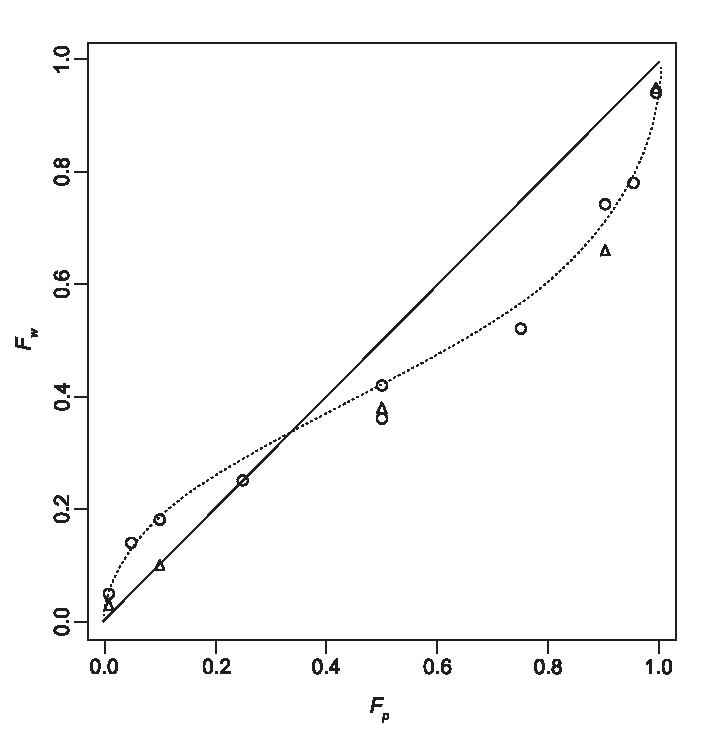
\includegraphics[width=.9\textwidth]{../../figs/TK1992.pdf}
% \end{center}

\parencite[p. 310, Fig. 1,relabelled axes]{TverskyKahneman1992}

\column{0.5\textwidth}
\begin{itemize}
  \item low probabilities treated as higher $\rightarrow$ high probabilities treated as lower
  \item stable empirical pattern: inverse-S shape
\end{itemize}

\red{Received wisdom:}
\bi
	\item	\red{PW = maladaptive irrational cognitive bias}
\ei

\begin{block}{In search of a mechanism}
	\begin{itemize}
	  \item[$\hookrightarrow$] How does this pattern emerge?
  	\item[$\hookrightarrow$] Can we derive a functional form\\ 
	(rather than fit a function)?
	\end{itemize}
\end{block}

\end{columns}
\end{frame}

\begin{frame}{Setup}
\begin{center}
Task: model payout, $x$, of a gamble as a random variable.
\end{center}
\begin{columns}[T]
\column{0.5\textwidth}
	\centering
	\textbf{Disinterested Observer (DO)} \\
	\vspace{0.5em}
	\includegraphics[height=3cm]{img/TverskyKahnemanFunny} \\
	\vspace{0.5em}
\column{0.5\textwidth}
	\centering
	\textbf{Decision Maker (DM)} \\
	\vspace{0.5em}
	\includegraphics[height=3cm]{img/LabRat} \\
	\vspace{0.5em}
\end{columns}

\begin{columns}[T]
\column{0.05\textwidth}
\column{0.35\textwidth}
	\vspace{0.5em}
% 	\centering
	DO assigns\\
	\red{probabilities $p(x)$} \\
  \red{CDF $F_p(x)$}\\
\column{0.2\textwidth}
% \centering
% 	\includegraphics[height=3cm]{img/coinflip}
\column{0.4\textwidth}
	\vspace{0.5em}
% 	\centering
  DM assigns different\\
  \blue{probabilities $w(x)$ (decision weights)}\\
   \blue{CDF $F_w(x)$}\\
\end{columns}
\end{frame}

% \section{Location and Scale of PDFs}
% \hyperlink{t-distribution}{\beamergotobutton{HTD}}
% Transmission of different uncertainties from PDFs into CDFs}

\begin{frame}{Possible model differences}{Locations, Scales, Shapes}
\centering
	\includegraphics[width=0.75\textwidth]{../../figs/2GaussianPDFs2Scales2Locations.pdf}
	\includegraphics[width=0.38\textwidth]{../../figs/pdfs_diff_scale_and_loc.pdf}
\end{frame}

% \begin{frame}{The Simplest Case : Different Scales}
% Numerically, our procedure can be applied to arbitrary distributions:
% \begin{enumerate}
% 	\item construct a list of values for the CDF assumed by the DO, \red{$F_p(x)$}
% 	\item construct a list of values for the CDF assumed by the DM, \blue{$F_w(x)$}
% 	\item plot \blue{$F_w(x)$} \vs \red{$F_p(x)$}
% \end{enumerate}
% \vspace{2em}
% \end{frame}

\begin{frame}{Thought experiment: DM assumes greater scale}
\centering
\begin{columns}%[T]
\column{0.35\textwidth}
% Add figures.\\
% 1. Two PDFs\\
	\includegraphics[width=\textwidth]{../../figs/2GaussianPDFs2Scales.pdf} \\
\column{0.65\textwidth}
% \vfill \\
Numerically easy for any pair of distributions (models):
\begin{enumerate}
	\item list values of DO's CDF, \red{$F_p(x)$}, at set ${x_i}$
	\item list values of DM's CDF, \blue{$F_w(x)$}, at same ${x_i}$
	\item plot \blue{$F_w(x)$} \vs \red{$F_p(x)$}
\end{enumerate}
% \vfill
\end{columns}

% 2. Corresponding CDFs\\
\only<2>{
	\includegraphics[width=.8\textwidth]{../../figs/mapping_cdfs_noarrows.pdf} \\
	}
% 3. Add arrows to CDFs\\
\only<3>{
	\includegraphics[width=0.8\textwidth]{../../figs/mapping_cdfs_1arrow.pdf} \\
	}
% 4. Explain how to transform to get to inverse S (add label to red line)\\
\only<4>{
	\includegraphics[width=0.8\textwidth]{../../figs/mapping_cdfs_2arrows.pdf} \\
	}
\only<5>{
	\includegraphics[width=0.8\textwidth]{../../figs/mapping_cdfs_3arrows.pdf} \\
	}
\only<6>{
	\includegraphics[width=0.8\textwidth]{../../figs/mapping_cdfs_4arrows.pdf} \\
	}
\only<7>{
	\includegraphics[width=0.8\textwidth]{../../figs/mapping_cdfs_5arrows.pdf} \\
	}
\only<8>{
	\includegraphics[width=0.8\textwidth]{../../figs/mapping_cdfs_6arrows.pdf} \\
	}
\only<9>{
	\includegraphics[width=0.8\textwidth]{../../figs/mapping_cdfs_7arrows.pdf} \\
	}
\only<10>{
	\includegraphics[width=0.8\textwidth]{../../figs/mapping_cdfs.pdf} \\
	}
\end{frame}

\begin{frame}{Applying the Procedure to the Uncertainty Types}
\centering
	\includegraphics[width=0.75\textwidth]{../../figs/Gauss_scale_location_both_KT.pdf}
	\label{LocationScale}
\end{frame}

% \begin{frame}
% \begin{columns}[T]
% \column{0.35\textwidth}
% \centering
% 	\includegraphics[width=\textwidth]{../../figs/2GaussianPDFs2Scales.pdf}
% \column{0.65\textwidth}
% Numerically easy for any pair of distributions (models):
% \begin{enumerate}
% 	\item list values of DO's CDF, \red{$F_p(x)$}, at set ${x_i}$
% 	\item list values of DM's CDF, \blue{$F_w(x)$}, at same ${x_i}$
% 	\item plot \blue{$F_w(x)$} \vs \red{$F_p(x)$}
% \end{enumerate}
% \end{columns}
% 
% Add graphic here to illustrate. For example dynamically: pick ten values of $x$, evaluate CDFs there (one by one), fill a list, plot CDFs against each other.
% \end{frame}

\begin{frame}{Interim conclusion}
\bi
	\item DM's greater scale gives inverse-S shape (unimodal distributions)
	\item difference in locations gives asymmetry
	\item reproduces observations of probability weighting
	\item[]
	\item[] \textit{Job done. Thank you for your attention ;)}
	\hfill
	\hyperlink{FunctionalForms}{\beamergotobutton{Functional Forms}}
	\label{InterimConclusion}
\ei
	\vspace{2em}
	\centering
	\includegraphics[width=0.8\textwidth]{../../figs/Our_result_LocScale_vs_KT.pdf}
\end{frame}

\section{Ergodicity Question}

\begin{frame}{The Ergodicity Question}
\begin{columns}[T]
\column{.35\textwidth}
	\bc \textbf{Typical DO concern} \ec
	What happens on average to the \red{ensemble} of subjects?
\column{.02\textwidth}
\centering \vspace{4em}  \red{\large $\neq$}
\column{.35\textwidth}
	\bc \textbf{Typical DM concern} \ec
	What happens to me \\
	\blue{on average over time}?
\end{columns}
\end{frame}


\section{Estimation}
\begin{frame}{Why DM's greater scale?}

%DM's adaptive rationality: err on the side of caution:
\begin{itemize}
  \item DM has no control over experiment
  \item experiment may be unclear to DM
  \item DM may not trust DO
%	\item uncertain outcome is consequential only to the DM,
% 	\item DM's ignorance,
  \item \ldots
\end{itemize}
\end{frame}

\begin{frame}{Experiencing probabilities}

\begin{itemize}
%  \item ``probability'' is polysemous \quelle{\parencite{Gigerenzer1991,Gigerenzer2018,HertwigGigerenzer1999}}
  \item probabilities are not observable
  \item DO encounters probabilities as known frequency in ensemble of experiments
  \item DM encounters probabilities as frequencies estimated over time

  \item[$\hookrightarrow$] \textbf{DM usually has to account for uncertainty in probabilities}
\end{itemize}
\end{frame}


\begin{frame}{Estimating probabilities}
\begin{columns}[T]
\column{0.5\textwidth}
\textbf{Rare Event} %\hfill \includegraphics[height=1.5cm]{img/BlackSwan} \hfill
\begin{itemize}
  \item $p(x) = 0.0001$
  \item \num{10000} observations
  \item $\sim 99.5\%$ of such time series will contain 0 or 1 events
  \item Na\"ive estimation: $\phat(x) = 0$ or $\phat(x)=0.0001$
  \item[$\hookrightarrow$] either impossible or 1000\% (over)estimation
\end{itemize}
\column{0.5\textwidth}
\textbf{Common Event} %\hfill \includegraphics[height=1.5cm]{img/WhiteSwan}  \hfill
\begin{itemize}
  \item $p(x)=0.1$
  \item \num{10000} observations
  \item $\sim 99.5\%$ of time series would contain between 50 and 150 events,
  \item Na\"ive estimation: $0.05< \phat(x) <0.15$
  \item[]
  \item[$\hookrightarrow$] only $\approx 50\%$ error in $\phat(x)$
\end{itemize}
\end{columns}
\vspace{2em}
 \centering
$\hookrightarrow$ small $p(x)$, small count \\
$\hookrightarrow$ small count, big uncertainty
\end{frame}

\begin{frame}{Relative estimation error is large for rare events}

\begin{center}
\begin{table}[!htb]
  \begin{tabular}{@{}ccccc@{}}
\toprule[2pt]
\makecell{Asymptotic\\probability} & \makecell{Most likely\\count} & \makecell{Standard error\\in count} & \makecell{Standard error\\in probability} & \makecell{Relative error\\in probability}\\
\midrule[2pt]
% .5 &	5000 & 71	& 0.01 & 0.71\%\\
0.1 & 1000 & 32 & 0.003 & 3\%\\
0.01 & 100 & 10 & 0.001 & 10\%\\
0.001 & 10 & 3 & 0.0003& 30\%\\
0.0001 & 1 & 1 & 0.0001 &100\%\\
\bottomrule[2pt]
\end{tabular}
\caption{$T = \num{10000}$, assuming Poisson statistics, relative estimation errors $\sim \nicefrac{1}{\sqrt{\text{count}}}$}
\label{errors}
\end{table}
\end{center}
\end{frame}

\begin{frame}{DMs don't like surprises}

To avoid surprises, let's say DMs add estimation uncertainty $err$ to every estimated probability, then normalize, s.t.

$w(x)=\frac{p(x)+\err{p(x)}}{\int \left(p(s)+\err{p(s)} \right)ds}$

This allows us to derive a functional form, \eg for the Gaussian case ... (find in manuscript)

...very similar to function chosen by Kahneman and Tversky.

Not sure we need much more. I'd just have one figure that gives a nice inverse S, for a Gaussian, say, based on estimation error.

\end{frame}

%\begin{frame}{Estimation of the decision weights}
%
%	Using the count $n(x)$ to form the best estimate and add to it the uncertainty about best estimate 
%	\begin{align}
%		w(x)						&\approx	\frac{n(x)}{T\delta x} \pm \frac{\sqrt{n(x)}}{T \delta x} \\
%		w(x)						&\approx	\phat(x) \pm \err{\phat(x)} 	\elabel{prob_est}
%	\end{align}
%	with the standard error expressed in terms of the estimate itself
%	\begin{align}
%		\err{\phat(x)}	&\equiv		\frac{\sqrt{n(x)}}{T \delta x} = \sqrt{\frac{\phat(x)}{T \delta x}} \\
%		\lim_{T\to\infty} w(x)	&\to p(x)					
%	\end{align}
%
%\end{frame}
%
%\begin{frame}
%\begin{center}
%  \includegraphics[width=.8\textwidth]{../../figs/dm_count_sim}
%\end{center}
%\end{frame}
%
%\begin{frame}
%\begin{center}
%	\includegraphics[width=.8\textwidth]{../../figs/square_root_error}
%\end{center}
%
%\end{frame}

% \begin{frame}{Simulation of the Estimation}
% \begin{center}
% 	\includegraphics[width=.65\textwidth]{img/dm_count_sim} \\
% 	$T = 100$, estimates of \red{$\phat(x)$} in red, estimates with one standard error \blue{$\phat(x) + \err{\phat(x)}$} in blue 
% \end{center}
% 
% \end{frame}
% 
% \begin{frame}
% 	Using the fact that $n(x)$ is a random variable itself, $n(x) \sim Poisson$, its fluctuations scale like $\sqrt{n(x)}$ \\
% 
% 	Using the count $n(x)$ to infer the asymptotic PDF as
% 	\begin{align}	  
% 		p(x)	&\approx \frac{n(x)}{T\delta x} \pm \frac{\sqrt{n(x)}}{T \delta x} \\
% 					&\approx \phat(x) \pm \err{\phat(x)}
% 	\elabel{prob_est}
% 	\end{align}
% 	with the standard error (expressed in terms of the estimate itself)
% 	$$\err{\phat(x)} \equiv \frac{\sqrt{n(x)}}{T \delta x} = \sqrt{\frac{\phat(x)}{T \delta x}}$$
% 	\bi
% 		\item standard error $\err{\phat(x)}$ shrinks as the probability decreases
% 		\item relative error in the estimate is $1/\sqrt{\phat(x)T\delta x}$ grows as the event becomes rarer
% 		\item consistent with our claim, that low probabilities come with larger relative errors
% 		\item[$\hookrightarrow$] Errors in probability estimates behave differently for low probabilities than for high probabilities: absolute errors are smaller for lower probabilities, but relative errors are larger
% 	\ei
% \end{frame}

\section{Conclusion}

\begin{frame}{Conclusion}
\lmlblue{Ergodicity Economics and probability weighting}
\begin{itemize}
  \item inverse-S shape appears as neutral indicator of a difference in opinion
%   \item relative probability estimation errors are greater for rarer events
	\item reported observations consistent with DM's extra uncertainty
	\item may arise from DM estimating probabilities over time
  \item[$\hookrightarrow$] Probability weighting is rational cautious behaviour under uncertainty over time
  \item[]
  \item See full paper at \url{bit.ly/lml-pw-r1}
  \item links to play with the code are inside
%   \\ \fullcite{PetersETAL2020R1}
% 	\item See blog post for the basic reasoning \fullcite{Peters2020}
% 	\item See blog post for the basic reasoning \fullcite{Buchanan2020}
\end{itemize}

\end{frame}
